
% TODO: get material from first year report 
%% TODO: furnish discussions and introduction throughout thesis with new citations from intro..


\section{Motivation}
\label{sec:intro_motivation}

%An ecosystem is a subset of the \emph{biosphere} - the entirety of the living systems on this planet. These biological systems are closely coupled, in a two way relationship, to the abiotic systems of the planet to such an extent that Lovelock, and other proponents of the \emph{Gaia theory}, suggest that the biotic and abiotic components together form a single homeostatic system which maintains conditions that are harmonious to life. In the strongest version of the theory the planet itself is a living system. This is not the place to argue for or against the theory, but regardless of its validity it remains undeniable that living systems generate significant effects at a planetary scale[REFS]. Humans, as one component of the biosphere, are fairly unique not only in the extent of their impact on planetary systems, but also their \emph{potential ability} to make reasoned decisions about collective actions based on knowledge of their impact. Given that the rate of species extinctions in the last century has been conservatively estimated at between 8 and 100 times the background extinction rate  \cite{ceballos2015accelerated}, and that the major drivers for these extinctions are anthropogenic [REF], it is abundantly clear that humans are failing to realise the aforementioned potential. Arguably the main reason for this failure is the systems of organisation..hard to make reasoned decisions when don't have sound theory!..but also lack of understanding about how ecosystems function..Second paragraph on stewardship, conservation and restoration..  This is my reason for studying the field of ecology....

An ecosystem is a subset of the \emph{biosphere} - the entirety of the living systems on this planet. Ecosystems are of fundamental importance to humanity because the multitude of services they provide support human civilisation  \cite{assessment2005ecosystems}. Additionally living systems are closely coupled, in a two way relationship, to the abiotic systems of the planet. Lovelock, and other proponents of the \emph{Gaia theory} \cite{lovelock1974atmospheric}, suggest that these biotic and abiotic components together form a single homoeostatic system which maintains conditions that are harmonious to life. Regardless of the validity of this theory, it has become increasingly clear that human activity is currently changing these global (biotitc and abiotic) systems. It is well established that the recent increase in global temperatures is anthropogenic \cite{pachauri2015synthesis,staudt2007understanding}. Furthermore is has been conservatively estimated that the rate of species extinctions during the last century was between 8 and 100 times the background extinction rate \cite{ceballos2015accelerated}. This elevated extinction rate is undeniably related to human activities, with land-use-change and loss of habitat cited as the primary causes \cite{foley2005global,newbold2015global}. Therefore studies into the detailed effects of habitat loss, and into the development of ecological theory in general, are urgently required in order to mitigate the effects of this \emph{biodiversity crisis}. Together such studies represent a body of knowledge with important implications for conservation, restoration and ecological stewardship.

%, and that the major drivers for these extinctions are anthropogenic [REF], it is abundantly clear that humans are failing to realise the aforementioned potential. Arguably the main reason for this failure is the systems of organisation..hard to make reasoned decisions when don't have sound theory!..but also lack of understanding about how ecosystems function..Second paragraph on stewardship, conservation and restoration..  This is my reason for studying the field of ecology....


%Habitat loss/alteration and climate change as the main anthropogenic drivers..Focus here on habitat loss. Community ecology - tools for the study of localised groups of species. Computational approach - hypothesis generation - defend bottom-up modelling of complex systems - make clear what it can and cannot do..

The breadth and scale of human impact on ecological systems is in itself sufficient motivation for this thesis. Much work has been done already in this area but, as we shall see, many questions remain open. In particular the dynamics and structure of \emph{hybrid-ecological communities} - collections of species that interact in diverse ways - are relatively unstudied \cite{kefi2012more,fontaine2011ecological}. Furthermore, the response of such communities to habitat loss has not yet been considered. In general, several recent studies have highlighted the importance of subtle and underlying changes to the structure of ecosystems that result from habitat loss, and which precede species extinctions \cite{tylianakis2007habitat,sole2006ecological,laliberte2010deforestation,albrecht2007interaction,spiesman2013habitat,hagen2012biodiversity,gonzalez2011disentangled}. As we shall see the field is moving beyond a focus on species extinctions only, towards a more detailed understanding of these underlying structural changes. In this thesis we conduct a number of experiments, using computer simulations, that aim to contribute to this understanding. Particular attention is paid to the role of species interactions in generating observable patterns, and in mediating the effects of habitat loss. \emph{In silico} investigations such as this are a useful tool in the development of ecological theory. However, their scope and interpretation must not be misunderstood (see section \ref{sec:intro_computers}). In the current chapter we present an overview of the literature that is relevant to the investigation, but before departing on that journey it is necessary to explain the context of the project as a whole.

This work is funded by the Bristol Centre for Complexity Sciences (BCCS). Therefore the content of the thesis falls under that generously sized umbrella term - \emph{complexity science} - which may leave some readers perplexed. They would not be to blame, especially given that the project motivation just provided rests on real-world \emph{ecological} concerns. Complexity science may be understood as the study of \emph{complex systems}. Ladyman, Lammbert and Weisner review the various definitions of a complex system \cite{ladyman2013complex}. They attempt to synthesise a concrete definition of this concept, which they argue has previously been rather loosely and carelessly applied. The authors arrive at the following tentative  definition of physical complexity:
\begin{quotation}
\emph{"A  complex  system  is  an  ensemble  of  many  elements which are interacting in a disordered way, resulting in robust organisation and memory."}
\end{quotation}
They assert that this definition contains conditions necessary, but perhaps not sufficient for complexity, and propose an alternative \emph{data driven} definition under which a complex system is one that generates data with a high measure of statistical complexity \cite{crutchfield1989inferring}. Indeed to define a complex system is no easy task. Depending on who you ask there may be further necessary conditions such as \emph{emergence}, \emph{hierarchical organisation}, \emph{de-centralised control} and even anti-reductionist properties such as \emph{top-down causation}. 

Given the lack of a concrete definition of complex systems, many of my contemporaries prefer a more \emph{pragmatic approach} to the question - what is complexity science? A fair summary of the consensus view is that complexity science represents a broad set of mathematical and computational tools which find application in increasingly diverse areas of the natural and social sciences. This expansion is driven by the ever increasing availability of data; advances in high performance computing; and the development of the tools themselves. For some the tools used, and the fields of study in which they find use, are too disjoint to call complexity science a unified field. This pragmatic approach is not dissimilar to the \emph{instrumentalist}, or "shut-up-and-calculate", interpretation of quantum mechanics \cite{norris2002quantum}, which finds popular support in the face of the difficult and unresolved philosophical questions posed by that theory. Further discussion on the nature of complexity is not relevant to this thesis, other than to say that if a general definition of a complex system were arrived at, then its criteria may be met by the concept of the \emph{ecological community}.

%(if concerned with the question at all)
% We now introduce key areas of theory??
  
\section{Community ecology}
\label{sec:intro_community_ecology}

%In fact the assertion that an ecological community represents a complex system is not beyond question. We consider the issue here, and in doing so we introduce the field of \emph{community ecology}. The field itself is well developed, with a vast body of literature, such that a comprehensive overview is beyond the scope of this thesis. Numerous references throughout this section may provide the reader with further insight into the main areas of interest.   

An ecological community may be broadly defined as a collection of species that coexist in time and space. The study of these collections, \emph{community ecology}, attempts to understand their structure, dynamics and function. A fundamental tenet in the field is that coexisting species interact with one another. This multitude of interactions gives rise to a \emph{tangled web} of inter-dependence between species, that ecologists have been aware of at least since the time of Charles Darwin \cite{darwin2009origin} (see quote in front matter), and probably long before. The interactions occur locally between individual members of species (e.g. two rabbits mate, one rabbit is eaten by	 a fox) in a manner that is arguably \emph{disordered}. On a larger scale robust patterns of organisation exist, in particular the biodiversity patterns of species richness and abundances \cite{sanderson2015patterns, purves2005ecological}. Therefore it is tempting to conclude that the ecological community fits the definition of physical complexity quoted in the previous section. %However the issue is not so easily resolved.

Perhaps the key question is whether large scale community patterns do in fact result from low level mechanics, such as the interactions between individuals. This question has been an ongoing source of debate. Numerous studies have suggested that empirically observed biodiversity patterns may be consistent with \emph{random} models of community assembly. In particular \emph{neutral theories of biodiversity} \cite{hubbell2001unified,volkov2003neutral} assert that the species in a community are functionally identical, or at least that any difference between species is \emph{neutral} with regards to their fitness. The fact that such neutral models are able to predict aggregate community patterns appears to reduce the complexity the system. As stated by Purves et al. \cite{purves2005ecological}, in a truly neutral community all species may be replaced by a single species without loss of community function. In such a case all biodiversity patterns are meaningless artefacts of randomness. However, empirical observations tell us that species are not functionally identical, instead they display differential traits. Purves et al. give the example of carbon uptake and storage in a forest. Trees have different life cycles (growth and decay rates especially), and therefore they display functionally different temporal profiles of carbon sequestration. As such, altering the species composition of the tree community, will alter the \emph{function} of the community (at least in terms of carbon storage, but most likely in other ways too). Therefore even proponents of \emph{neutral} theories cannot claim that they explain it all. \replaced{Rather}{In general } neutrality \added{may} provide\deleted{s} useful \emph{null models} against which to test the relative importance of other factors \deleted{, such as species interactions,} in shaping communities. \added{It seems that community assembly in nature is driven by a combination neutral and non-neutral processes \cite{purves2005ecological,staniczenko2014selecting}. Therefore departures from neutrality are likely (although not necessarily \cite{purves2005ecological,bluthgen2008interaction}) indicative of non-random and therefore ecologically meaningful mechanisms.}  

%.this can be seen on a global scale..Also functionally species are distinct - refer to the example of a forest with carbon uptake..In reality communities are likely to be some combination of neutral and structured..(Do not try to resolve the debate! Just introduce it and say that it is relevant to our modelling framework, and the questions we can asnwer using it.)

%(Specialistion, generality, moropholigical differecnes, pollination as an ecosystem service..)

In general, the consensus view is that species interactions\added{, and the non-random patterns that they form,} do play a role in community assembly. Strong support for the influence of species interactions on community structure comes in the form of empirically observed \emph{trophic cascades} \cite{knight2005trophic,ripple2012trophic}. A trophic interaction is one in which energy is transferred between the interacting partners. Food webs and food chains represent collections of species interacting in such a way. The connectivity in these systems means that an action which influences one species may have knock-on effects on the other species. Consider a simple three species food chain, in which grass is eaten by rabbits, which in turn are eaten by foxes. Grass represents the \emph{basal trophic level} and is the sole source of all energy is this system, being the only \emph{auto-trophic} species. If all grass is removed from the system the species in higher trophic levels go extinct: both the rabbits, and indirectly the foxes, will starve. This is a \emph{bottom up} trophic cascade. Alternatively an action may be taken which benefits the fox population. An increased numbers of foxes is likely to have \emph{top-down} cascading effects. For example, more foxes means fewer rabbits, which in turn means more grass. Clearly there is a dynamic element to any such changes, as we shall see throughout this thesis. 

The reintroduction of wolves into Yellowstone National Park is perhaps the most famous example of a real-world trophic cascade. The grey wolf (\emph{Canis lupus}) was reintroduced to Yellowstone in 1995. Analysis by Ripple and Beschta  \cite{ripple2012trophic} suggests that the abundance of mature aspen and cottonwood trees increased during the following 15 years, and attributed this increase to a reduction in elk numbers due to predation by wolves. They also noted an increase in beaver and bison numbers, which they speculate resulted from reduced competition for resources with the elk. However, the observed changes displayed a spatial pattern. Specifically they recorded differences in the response to wolf reintroduction between the southern and northern regions of the park, and between highland and riparian (riverside) areas. Subsequent research \cite{marshall2014interactions} supports the existence of a trophic cascade in Yellowstone, but highlights the importance of other factors, such as landscape heterogeneity and environmental conditions, in determining its effect. From this we conclude that species interactions can indeed play an important role in ecology, but that their effects cannot be fully understood in isolation.

\begin{figure}
	\centering
	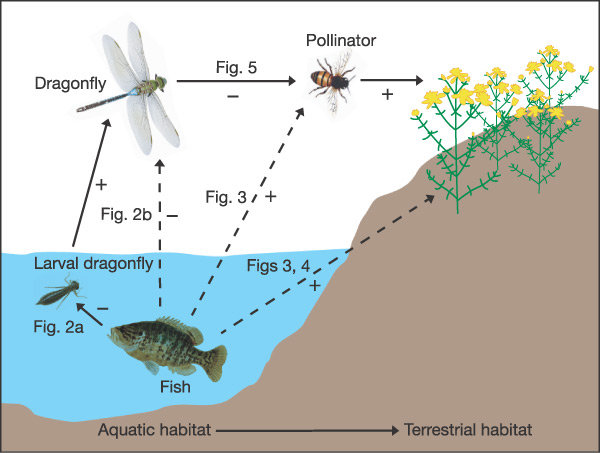
\includegraphics[width=0.6\textwidth]{{{diagrams/natureKnight}}}
	\caption[A trophic cascade.]{\textbf{An example of a trophic cascade} that crosses community boundaries. The presence of fish in ponds was empirically determined to indirectly benefit plant reproduction in neighbouring communities. Figure reproduced from Knight et al. \cite{knight2005trophic}.}
	\label{fig:trop_casc}
\end{figure}

Another informative example of a trophic cascade was published by Knight et al. \cite{knight2005trophic}. In their study it was shown that the presence of fish in pond communities can indirectly facilitate plant reproduction in neighbouring terrestrial communities. The pathway of influence is depicted in figure \ref{fig:trop_casc}. Fish feed on dragonfly larvae in ponds, reducing the number of adult dragonflies which predate on pollinators. The presence of fish was shown to measurably benefit nearby plants by increasing pollination rates. This example again highlights the importance of species interactions, but carries with it a warning to the community ecologist. The definition of a community as an object of study (given at the beginning of this section) requires a delineation according to spatial scale or habitat type. From \cite{knight2005trophic} it is clear that such a delineation can prove problematic because communities may influence one another. The pathways of influence are not confined to species with complex life histories, such as the dragonfly. More simply communities may influence one another via dispersal and immigration: the movement of individuals throughout space.

It is necessary to be aware of the limitations faced when focusing on a \emph{local} community. Ricklefs argues \cite{ricklefs2008disintegration} that the ecological community is an \emph{epiphenomenon}, and that the strong focus of ecologists on local collections of species has hindered progress in our understanding of biodiversity at regional scales. Certainly spatial considerations are fundamental to our understanding of ecology. Whittaker showed that the concept of \emph{biodiversity} must be considered on different spatial scales \cite{whittaker2001scale}, and it is well known that \emph{species richness} (simply the number of species present) scales with spatial area \cite{rosenzweig1995species}. More recently it has been shown that the choice of spatial scale also affects calculations of stability. Wang and Loreau \cite{wang2014ecosystem} demonstrated empirically that temporal variability in biomass can decrease with spatial scale, possibility due to averaging over asynchronous fluctuations at the landscape level. 

In general we see that the ecological community is an abstraction of nature, that is sensitive to spatial scale. Geographic boundaries may exist which validate this abstraction. For example islands present useful study systems of relatively isolated natural communities. However, in most cases the consideration of multiple spatial scales leads naturally to the concept of the meta-community \cite{leibold2004metacommunity}. At the landscape level one may think of a number of interacting communities, where local assemblages of species are connected via the dispersal of individuals. Meta-community modelling has increased in popularity \cite{leibold2004metacommunity,logue2011empirical}, and provides an important link between the local and the regional scales. However, such models tend to use a simplistic representation of the local community (e.g. \cite{klausmeier2001habitat}). Generally each locality is represented as a patch, containing information on species abundances but no spatial structure. Therefore meta-community modelling represents a trade-off in resolution at different spatial scales. For this reason \emph{community modelling} remains useful for understanding the details of local dynamics and structure, but we must be aware of the wider context in which the local community exists. 

%More importantly spatial processes 

%There is some truth in this.. Consideration of spatial scales has provided hey insights into our understanding of biodiversity \cite{}, and more recently into ecosystem stability \cite{}. 

%Consciousness as an epiphenomenon, soci-cultural landscape..still valid object of study..provided understand context. We assert that community is a complex system, and is worthy of study..but that to be useful any results must be syntehsised with other areas..

%The discussion above leads us to define the scope of the current thesis. The project represents a computational investigation of ecological communities. 

%However the question of scale ...

%\cite{ricklefs2008disintegration}
%Species spatial ranges - not explained by local focus..meta-community theory..
%The field is too large to give a coherent overview. In this section we introduce some keys themes from community ecology that are relevant to the current project. 


%This inter-dependence between species can make communities sensitive to perturbation - if a species, upon which another species is strongly dependent, goes extinct it is likely that the dependant species will be lost also. These \emph{co-extinctions} and other knock-on effects, such as \emph{trophic cascades}, have been empirically observed \cite{knight2005trophic,ripple2012trophic}, giving evidence to the importance of species interactions in shaping communities.   However the tangled web may also generate communities which are remarkably robust to perturbation, and which persist through time despite varying environmental conditions. The story of community ecology has been one of trying to understand the general mechanisms and factors that shape communities, generating the observed patterns of biodiversity. This task is far from complete, and urgently required given the crisis facing life on this planet.

%Mention metacommunities? - and IBT (referred to here from conclusion in chapter 3) And summary on persistence - put more refs here on stabilising role of dispersal..
%
%In general the field holds the belief the species interactions play an important role in the community, although an explicit and complete understanding of \emph{how} they do remains to be achieved (or may never be). 
% following the tenet that these three properties are related (see section \ref{sec:intro_role_of_sturcture}). A general theme in community ecology has been to look for

%Importance of networks..interactions..archetypal complex system (definition form Ladyman?) where emergent properties are generated by the many interacting agents...Obviously other factors - environmental, abiotic..  

\subsection{Species interactions}
\label{sec:intro_interactions}

%\cite{o2009perturbations} - interaction strengths is focus, but also spatial stability. c.f. a,b,g stability and Lurgi et al.

In a local community, interactions occur between individual organisms. However, it is common to use a condensed representation by defining which \emph{species} interact. If the interacting individuals belong to the same species the interaction is referred to as \emph{intra-specific}; if they belong to different species it is referred to as \emph{inter-specific}. Inter-specific interactions broadly fall into three groups: \emph{antagonism}, \emph{mutualism} and \emph{competition}, based on the effect that each species has on the other. An antagonism is an interaction where there is benefit to one species and harm to the other. A mutualism benefits both parties, whereas a competition harms both parties. Whatever the type of interaction being studied, it is possible to represent the pattern of interactions between the species in the community as a network. Such a network may be referred to as a \emph{species interaction network}, or simply an interaction network, and they have proven a useful tool for community ecologists \cite{bascompte2007networks}. There is a widely held view that the \emph{structure} of these networks provides insight into the function and dynamics of ecological communities (see section \ref{sec:intro_role_of_sturcture}). Correspondingly an arsenal of network metrics have been developed, drawing on the mathematics of \emph{network theory}, with which ecologists attempt to characterise meaningful aspects of network structure. Several of these metrics are introduced in section \ref{sec:define_network_metrics}, and used in the analysis throughout the thesis.

It has been, and largely remains, common practice to define a community by the way in which its constituent species interact. So in addition to the spatial delineation already discussed, a delineation exists according to interaction type, such that studies may refer to \emph{antagonistic communities} \cite{albrecht2007interaction}, \emph{mutualistic communities} \cite{bascompte2007plant} or \emph{competitive communities} \cite{klausmeier2001habitat}. Antagonistic communities in the form of food webs are perhaps the most general since all non-basal species must feed in some manner, although studies of host-parasitoid communities are also common \cite{laliberte2010deforestation}. Mutualistic communities have received much attention in the form of plant-pollinator communities, given the key role of pollination as an ecosystem function that helps maintain plant biodiversity \cite{vanbergen2013threats}. However, in nature there exists no clear delineation based on interaction type. It is possible for all types of interaction to occur between species that co-exist in time and space. Therefore there has been a recent move towards studies of communities that contain multiple types of interaction, or \emph{hybrid communities} \cite{sauve2014structure,kefi2012more,fontaine2011ecological,evans2013robustness,montoya2015functional,mougi2012diversity}. Some of these studies have brought into question previous results derived from communities with single interaction types (see section \ref{sec:intro_role_of_sturcture}), and so represent an important development in the field.

Another recent development is the quantification of \emph{interaction strengths} in ecological network studies. Early network metrics used by ecologists were based on binary networks \cite{bersier2002quantitative}, i.e. networks without weights associated with the links. This is in part because it is easier to empirically identify the presence of an interaction (to define the existence of a link in the network), than it is to quantify the strength of the interaction (to define the weight of that link). However, metrics have since been developed that incorporate interaction strength \cite{bersier2002quantitative,bluthgen2008interaction,bluthgen2006measuring} and several studies have highlighted the improved descriptive power of such \emph{quantitative network metrics} over their \emph{qualitative} counterparts (see sections \ref{sec:intro_role_of_sturcture} and \ref{sec:intro_empirical_HL}). A key feature of ecological networks is their propensity to contain a few strong interactions and many weak interactions. Qualitative descriptors do not capture this structural feature \cite{bersier2002quantitative}. It is common in empirical studies to use the \emph{observed frequency} of an interaction as a proxy for its strength \cite{bluthgen2008interaction,berlow2004interaction}. In many cases this interaction frequency is a good approximation of the biomass flow or energy transfer along a trophic link, and therefore serves as a useful measure for how important that link is in the network. However, other metrics may be used to quantify link weight. For example plant-pollinator studies may measure pollen transport in order to quantify the amount of pollen that `flows' along each interaction pathway \cite{devoto2011night}.  

There are many reasons to \emph{quantify interaction strengths}, aside from the assignment of link weights to interaction networks. Strong interactions between species are thought to be destabilising for a community. A seminal theoretical study on this topic is May's 1973 paper \cite{may1972will}. Using \emph{random matrix theory} he derived results on the dynamic stability of interaction networks with random link weights. Specifically the weights were assigned randomly from a distribution with mean zero and variance $\sigma^2$. May concluded that the probability for such a system to be dynamically stable (in terms of the linear stability of the equilibrium) decreased with $\sigma^2$, and also with the \emph{connectance} C (the fraction of non-zero link weights in the full coupling matrix). Subsequently a number of theoretical studies confirmed that strong interactions are destabilising in food webs \cite{mccann1998weak,gross2009generalized}, and the effect has been empirically observed by O'Gormann \cite{o2009perturbations}.  From a dynamical systems perspective this result is intuitive. Strong coupling increases the dependence between variables. From a practical perspective the result is significant because by quantifying interaction strengths we may understand aspects of community stability. 

Returning to the example of trophic cascades, we see further motivation for quantifying interaction strengths. In the case of the \emph{Yellowstone cascade}, we may want to quantify the effect that a change in one population (wolves) has on the populations of other species (elk, aspen, bison, beavers). This is one definition of interaction strength, and we have seen that in Yellowstone it was spatially dependent. Similarly one may want to determine the effect that the removal of one species would have on a community. Extinction of one species may result in cascading extinctions \cite{evans2013robustness}, which are likely determined by interaction strengths \cite{eklof2006species,kaiser2010robustness}. Extensive reviews on the subject of interaction strengths are provided in \cite{berlow2004interaction,wootton2005measurement}.  A general theme emerging from the two papers is that methods (both empirical and theoretical) for quantifying interaction strength are dependent on the question being asked. Various methods capture different aspects of the effect of one species on another, and any two metrics are not necessarily comparable. Wootton and Emmerson \cite{wootton2005measurement} in particular call for more clarity from researchers on the metrics being used, and for an improved dialogue being theorists and empiricists regarding the issue of interaction strengths. In this thesis interaction strengths play a central role. The way in which they are defined is discussed in section \ref{sec:define_network_metrics}, and revisited in chapter \ref{chap:interactions}.


% As discussed by Wootton and Emmerson \cite{} there are numerous reasons to quantify interaction strengths, and correspondingly there exists a wealth of definitions and metrics for doing so. Their paper, together with that of Berlow et al. \cite{}, provides a fairly comprehensive overview of the subject. 
 % researchers should provide more clarity on the metric being used for interaction strength, and the reasons for doing so. Such clarity would avoid erroneous conflation of results from unrelated studies. Furthermore both papers emphasise the need for an improved synthesis of empirical and theoretical results regarding species interaction strengths. Since species interaction strengths represent central topic of this thesis, we consider two examples to highlight some of the issues in this area.

%A further example highlights the potential disparity between empirical and theoretical concepts of interaction %strength. Trophic cacade..context dependent?
%\cite{tylianakis2007habitat} 
%\cite{gibson2011sampling}

%
%s
%
% Such interactions may easily be represented as a network, which codifies the pattern of interactions between the species in a community. This is useful because tools taken from network science, and developed specifically for application in community ecology, may be used to analyse the community (see section [REFS] for more details on these methods). There are various conventions used for the network representation, but all of them use some kind of interaction or \emph{community matrix}. We will call this matrix $\mathbf{A}$ such that the elements $a_{ij}$ give some measure of the effect that species $j$ has on species $i$. Therefore a two species predator-prey system may be represented as:
%\begin{equation}
%A = 
%\begin{pmatrix}
%0 & -1 \\
%1 & 0
%\end{pmatrix},
%\label{eq:example_adj}
%\end{equation}
%where it is clear that species 1 is the predator since it has a negative impact on species 0 ($a_{01}<0$), whilst receiving benefit itself ($a_{10}>0$). Notably here $a_{00}$ and $a_{11}$ represent intra-specific interactions, or self-loops in the network, which may be non-zero due to mechanisms such as competition for space, predator-interference, or Allee effects [REFS]. In this representation the matrix is binary, and therefore the network is directed but unweighted. Conventionally ecologists have used unweighted networks since it is much easier to identify the presence or absence of an interaction than it is to quantify its strength. 
%
%Therefore the `first wave' of ecological network metrics were developed without reference to interaction strengths, whereas subsequent quantitative metrics took interaction strength into account \cite{bersier2002quantitative}. Several studies highlighted the importance or quantitative metrics over qualitative ones. For example.. Interactions may also be classified as \emph{trophic} or non-trophic. Trophic interactions, such as predation, represent a directional flow of energy from one species to another. Therefore a food web can be thought of as a map of trophic energy or biomass flows through a community. In such case the link weight can take the natural units of energy flow rate, although this is not necessarily easy to measure. It is common in empirical studies to use the observed frequency of interaction as a proxy for the interaction strength. This is reasonable - if lynx are observed to prey on hares more frequently than on lemmings, then we may conclude that there is more biomass flow along one pathway than the other. Similar procedure are applied to pollination a mutualistic interaction which is also trophic..However the measurement of interaction strength is not simple, and as discussed by Berlow \cite{berlow2004interaction} there is no single definition or method. (return to this issue)
%
%In nature all the types of interaction mentioned above have the potential to coexist. In fact it is not necessarily clear which interaction belong to which type. For example the interaction between a bee and a flower is trophic - the bee takes nectar from the plant. This has an energetic cost to the plant. There is also the potential for benefit to the plant since it may be pollinated, and also gives up pollen which will later go on to pollinate a mate. Therefore we expect the species in a single community to be engaged in multiple interaction types. Until recently most community ecology has focused on single interaction types in isolation. - that is they have studies subsets of the full community. So, for example, pollination studies have sampled interactions between plants and pollinators to construct mutualistic networks \cite{gibson2011sampling}, whilst parasitism studies have sampled rates of parasitism on each host to construct antagonistic networks \cite{tylianakis2007habitat}. It is also worth noting here that such focus on single interaction types has often meant that the network being studies is \emph{bipartite} - i.e. one type of species linked to another via the interaction in question (host-parasitoid, plant-pollinator etc.) The single interaction focus has generated interesting results on the structure and functioning of such networks and sub-communities (see section \ref{sec:intro_role_of_sturcture}). However more recently there has a move towards integration of multiple interaction types as they are found in nature.        
%
%(Worth noting that May's classic study involves multiple interaction types, other theoretical studies have..in stablity section?)
%
%(Include figure!)-Pocock or Kefi?

%\subsection{The role of network structure}
\label{sec:intro_role_of_sturcture}

%SEE DISCUSSION ON STABILITY IN (NOW DEPRICATED) CHAPTER 5!

Much work in community ecology has focused on the question: how does the structure of an interaction network relate to properties of the community. This is what we refer to as \emph{the role of network structure}. Community properties that may be related to network structure include stability, diversity (species richness and abundances), and ecosystem functions such as pollination and nutrient cycling. We focus here on work that relates structure to \emph{stability} because it is of particular relevance to the current project. In later chapters we will be interested in how community stability is affected by habitat loss. In depth treatments of the role of network structure on community properties in general are provided in \cite{thompson2012food} and \cite{rooney2012integrating}. As discussed in section \ref{sec:intro_interactions}, the metrics used to capture aspects of network structure are either qualitative or quantitative. Given that links weights represent a structural feature of weighted networks that provide more information about the system being studied, it seems natural to include link weights when that information is available. Bana{\v{s}}ek-Richter et al. \cite{banavsek2004sampling} have shown that quantitative network metrics generally provide more accurate representations of network structure when link weights are included. Correspondingly most ecological network studies now quantify link weights (interaction strengths) in some form.

%The belief that the pattern of interactions between species is relevant to properties observed at the community level is justified by a complex systems approach. If community properties result from local interactions between species, then the tools of network theory may used to derive meaningful information from the structure of the interaction network. 
%Much of community ecology focuses on this subject and tries to relate network structure to community properties, such as \emph{stability}, and to ecosystem functions, such as pollination and nutrient cycling. 

Community stability is a multifaceted and evolving concept \cite{lurgi2015effects,montoya2016invariability,arnoldi2015,wang2006inferring}, that includes aspects such as \emph{robustness}, \emph{persistence}, \emph{variability} and \emph{resilience}. These are discussed further in section \ref{sec:def_stability_metrics}, where definitions of associated metrics are provided. A general observation is that large and complex ecological communities can be remarkably stable given the extent of the external perturbations they face. There is an apparent contradiction between this empirical observation and some theoretical results regarding stability. May's work \cite{may1972will} showed that large and highly connected communities are unlikely to be stable. Subsequent work by Gross \cite{gross2009generalized} has shown that indeed the probability of obtaining a stable network \emph{at random} is vanishingly low for networks of many species ($P(stable) < 10^{-4}$ for networks of 50 species). Despite these theoretical results large and stable communities are observed in nature. Either there is something wrong with the way these studies compute stability, or there are some non-random properties of real-world network structures that confer stability on communities. \added{(A third possibility, discussed in section \ref{sec:def_stability_metrics}, is that the focus of theorists on stability is mistaken because communities in nature are in fact unstable.)} 
%(Need to work space and climate into the above discussion. Also include picture of hare-lynx food web? Use hare-lynx model fit plot form first year report?)

%Structure versus dynamics - refer to ODEs, simple example. Jacobian, relates to...

As we saw in section \ref{sec:intro_interactions} community ecology has historically focused on communities with single interaction types. This focus has produced results that connect structural properties with stability in such systems. For example it is well documented that \emph{compartmentalisation} promotes stability in antagonistic communities \cite{stouffer2011compartmentalization,thebault2010stability}. Conceptually compartmentalisation is the tendency for groups of species to interact strongly within the group, while interacting weakly with species outside the group. This property has been observed in empirical food webs \cite{stouffer2011compartmentalization}, suggesting that it may indeed play an important role in stabilising natural communities. Weak connectance \cite{may1972will,thebault2010stability} and high variability in interaction strengths \cite{van2016food, jansen2003complexity} have also been suggested to play a role. The structural properties of mutualistic communities appear to differ from those of antagonistic communities. Empirically it has been observed that mutualistic communities have a \emph{nested} structure \cite{bascompte2007plant}. Nestedness can be thought of as the tendency for specialist species to interact with subsets of the interaction partners of more generalist species. This concept is illustrated in figure \ref{fig:nested}. The property of nestedness has been shown to promote stability in mutualistic communities, as has high connectance \cite{thebault2010stability}. 

\begin{figure}
	\centering
	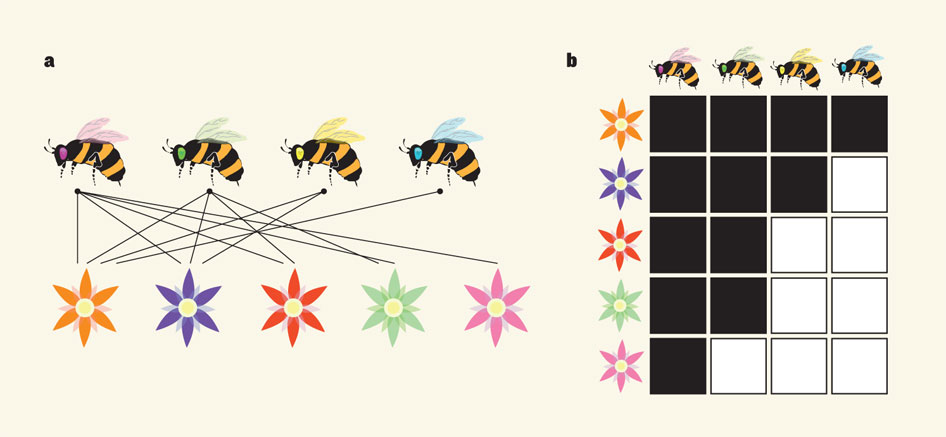
\includegraphics[width=0.7\textwidth]{{{diagrams/nest}}}
	\caption[Illustration of nestedness.]{\textbf{Nestedness} is the property that the diets of specialist species are subsets of the diets of generalist species. It is common in mutualistic communities. Figure reproduced from \cite{allesina2012ecology}: `\textbf{a}, In the mutualistic interactions that occur between plants and their pollinators, some species (generalists, such as the pink-eyed bee) interact with many partners, whereas other species (specialists, such as the blue-eyed bee) have few partners. \textbf{b}, Such networks have been described as `nested', as they produce a triangular pattern when the interactions (depicted by black squares) are arranged in a matrix. '}
	\label{fig:nested}
\end{figure}


However, more recent work on \emph{hybrid communities} by Sauve et al \cite{sauve2014structure} has brought into question some of the structural properties commonly associated with stability. They modelled communities comprising mutualistic and antagonistic interactions, and demonstrated that the effects of modularity and nestedness on stability were strongly reduced. This controversial finding indicates the importance of the recent push to study hybrid communities (previously discussed in section \ref{sec:intro_interactions}). It has also been shown, by Mougi et al. \cite{mougi2012diversity}, that the introduction of mutualism can stabilise antagonistic communities. The novelty of these results highlights how far there is to go in order to understand the role of different interaction types as they occur in nature: simultaneously. This thesis represents one step on that journey.

%Structure-stability : antagonism, mutualism, combined - general May, Thilo - does appear that structure plays a role, but this role is not yet understood - what is clear is that stability seems unlikely, and yet ecosystems appear stable - something fishy! The push to find structural properties that confer stability.. \cite{van2016food, jansen2003complexity}. Nestedness, mutualism etc.

%Thilo - variability in link strenghts promotes stability, 

%This may be a suitable place to touch on confusion regarding the term stability, and clear up some confusion...(robustness, different types of stability, persistence) - no refer forwards to section \ref{sec:def_stability_metrics}

%Structure vs function: ecosystems services and functions, pollination as the perfect example.
%Tylianakis involved in: \cite{thompson2012food}

%\subsection{Network generation}
%\label{sec:intro_net_gen}
%
%Empirical methods, frequency as a proxy for interaction strength. What is meant by interaction strength? What is relevant? (Refer forwards to final chapter, more detail in intro there). 
%
%Possible section: how are networks created - refers to the problem of estimating species interaction strengths and relating these to dynamics and function.
%
%Network inference - brief reference to methods for doing this, and why you would want to...


\section{Habitat loss}
\label{sec:intro_habitat_loss}

A significant portion of this thesis (chapters \ref{chap:habitat_loss_high_immigration} and \ref{chap:varying_immigration_rate}) is devoted to the study of community responses to habitat loss. As we saw in section \ref{sec:intro_motivation}, habitat loss is one of the leading causes of the extensive damage to ecosystems that we are witnessing globally. Therefore understanding the effects of habitat loss, and how to mitigate them, is more important now than ever. In this section we introduce the current state of knowledge regarding this issue, from a community ecology perspective. We cite certain key papers, however the field is too vast to provide a comprehensive overview. The reader is referred to reviews in \cite{hagen2012biodiversity} and \cite{gonzalez2011disentangled} for such information. In section \ref{sec:intro_modelling_HL} we outline how habitat loss has been modelled previously, and discuss the results of this modelling. In section \ref{sec:intro_empirical_HL} we then compare the modelling results to certain key empirical studies. In the literature a range of related concepts are studied, including \emph{habitat alteration}, \emph{degradation} and \emph{fragmentation}. In what follows we use \emph{habitat loss} to refer to all these concepts, except where a specific distinction is warranted.

In nature habitat may be destroyed in a number of ways. In general there is some spatial structure to the human activity that causes loss of habitat. Development often follows lines of infrastructure such as roads, which themselves represent linear loss of habitat. On a local scale, human activity is usually aggregated. Urban development is approximately contiguous, and agricultural land use is usually concentrated in certain areas. However, there is also a random element to the loss of habitat, particularity on a larger spatial scale. For example, the spatial distribution of exploitable resources (fertile land, mineral deposits etc.) is approximately random. Therefore we may consider there to be two extremes to the spatial pattern in which habitat is lost. At one end of the spectrum contiguous regions of habitat may be lost, leaving the rest of the landscape untouched. At the other extreme is habitat loss which is totally random, i.e. without spatial structure. In this thesis we consider \replaced{these two extreme cases. Throughout we shall refer to either random or contiguous habitat loss (see section \ref{sec:model_HL}). However, in section \ref{sec:} we consider some of the subtle interplay between these two cases.}{both extremes (see section \ref{sec:model_HL}).}

%Aside from this study there is a lack of empirical and theoretical results on the response of hybrid networks to habitat loss. This project aims to make a contribution towards this area. We will extend on the work of Lurgi et al. \cite{lurgi2015effects} to simulate multi-trophic communities with mutualistic and antagonistic interactions. By investigating the response of these communities to simulated habitat destruction we will be generating novel results and predictions which can be tested empirically in the future. To do this we will employ a range of metrics to quantify structural changes and community stability. We will focus on the regime before species are lost from the community, with an interest in the underlying changes that occur as a result of habitat destruction.

%\emph{duffy2003biodiversity} and \cite{raffaelli2004extinction} : higher trophic levels most vulnerable to HL (extinctions). \cite{dobson2006habitat} - same message `trophic collapse'

\subsection{Modelling studies}
\label{sec:intro_modelling_HL}
%(see Dani's list of refs.)

Historically studies of habitat loss have focused on species extinctions, since the loss of species is arguably the most visible consequence of any perturbation. Numerous theoretical studies have investigated how the species extinctions resulting from habitat loss depend on the spatial pattern of the perturbation \cite{allen2007self,jager2006simulated,dytham1995effect,
hill1999habitat,travis2003climate,with1999extinction,ovaskainen2002metapopulation}. The studies cited employ spatially explicit (either lattice-type or meta-community type) modelling, such that habitat can be destroyed according to different spatial patterns. In general these studies agree that species extinctions occur at a higher level of habitat loss when the destruction occurs in some spatially-correlated way, rather than at random. 

Other modelling has indicated that the loss of species is mediated by properties of the interaction network structure. Fortuna and Bascompte \cite{fortuna2006habitat} modelled the dynamics of mutualistic communities under habitat loss. They demonstrated that random network structures produced species extinctions at lower levels of habitat loss, compared to network structures empirically derived from real-world communities. Similarly Melian and Bascompte \cite{melian2002food} used a meta-community model to demonstrate that certain network properties can help to prevent extinctions in simulated antagonistic communities. Both increasing levels of omnivory, and reducing top-down control by predators were shown to increase extinction thresholds. However, both studies cited pertain to small model networks, and the results remain to be demonstrated empirically.     

Understanding the full effects of habitat loss on a community necessarily requires the consideration of multiple trophic levels \cite{dobson2006habitat,sole2006ecological}. We saw in section \ref{sec:intro_interactions} that changes to a single species in a community can have effects that cascade across trophic levels. Modelling by both Dobson et al. \cite{dobson2006habitat}, and by Sole and Montoya \cite{sole2006ecological}, suggests that species in higher trophic levels are most vulnerable to habitat loss. Dobson et al. describe how diversity, and associated ecosystem functions, are lost first from higher trophic levels. They refer to this effect as \emph{trophic collapse} of the community.

We have previously noted a move towards the study of hybrid communities with multiple types of interaction (section \ref{sec:intro_community_ecology}). Since this is a recent trend, such communities have yet to be studied extensively in the context of habitat loss. The only relevant study we are aware of at the time of writing is by Evans et al. \cite{evans2013robustness}. They empirically constructed a network of networks, spanning several habitats on a farm ecosystem and comprising multiple interaction types. A robustness algorithm was then used to determine how vulnerable the hybrid network was to the loss of different habitats from the farm. Interestingly they reported that two of the most important habitats, relative to their sizes, were hedgerow and wasteland. However, their approach was spatially implicit and did not consider the \emph{dynamics} of the farm community. \added{As we shall see, such an approach is insufficient for understanding the spatio-temporal effects of habitat loss (sections \ref{sec:}). Therefore a more detailed modelling treatment of hybrid-communities under habitat loss is required.}

Species extinctions are not the only effect of habitat loss on communities. Other effects may include changes in stability, in the distribution of species abundances and in network properties. These more subtle changes may be thought of, in some sense, as representing a decline in ecosystem `health', and a loss of ecosystem function, which may occur prior to the loss of any species. Of particular concern are changes in \emph{species interactions} resulting from habitat loss. We saw in section \ref{sec:intro_community_ecology} that species interactions play a key role in generating community patterns and maintaining ecosystem function. This led Janzen to comment in 1974 that, when considering the effects of deforestation

\begin{quote}
 \emph{``what escapes the eye, however, is a much more insidious kind of extinction: the extinction of ecological interactions''} \cite{janzen1974}.
\end{quote}
%
Modelling studies have investigated the loss of interactions due to habitat loss. For example Fortuna et al. \cite{fortuna2013habitat} used a meta-community model to show that mutualistic interactions may be lost rapidly beyond a critical threshold of habitat loss. \replaced{As we shall see in the following section, empirical studies have revealed that interaction networks may display structural changes in response to habitat loss. Such changes clearly result from the non-random loss of interactions between species. However, despite extensive empirical evidence for how interaction networks respond to habitat loss, theoretical models have yet to reproduce these effects. Therefore, by simulating multi-trophic community dynamics under habitat loss, we intend to reveal some of the low level mechanisms responsible for known structural changes (see section \ref{sec:scope}).}{However, we are not aware of any modelling that has attempted to reveal changes in network structure at the community level. Our knowledge of such changes under habitat loss comes from empirical studies.}

%Another novel aspect of this work is the spatially explicit modelling approach...
%And some of the spatial analysis employed...

%\cite{sole2006ecological}   - spatially explciti analyisis.

\subsection{Empirical studies}
\label{sec:intro_empirical_HL}

There are certain empirically observed responses to habitat loss that appear to be general. Namely habitat loss affects species in higher trophic levels more strongly than those in lower trophic levels \cite{duffy2003biodiversity,raffaelli2004extinction}, it is generally de-stabilising, and beyond a certain level of destruction it results in the loss of species \cite{gonzalez2011disentangled}. These effects are consistent with the theoretical studies cited in the previous section (\ref{sec:intro_modelling_HL}). \added{Another key theoretical result - that communities respond differently to random and correlated habitat loss - also has empirical support, although the situation is more complex in nature than in the simple models cited.} \deleted{Empirically studying the effect of the spatial pattern of habitat loss is a challenge because this requires controlled destruction.} \added{In empirical studies a distinction is often made between \emph{habitat fragmentation} and \emph{area loss} \cite{gavish2012decoupling}. In the context of this thesis we may broadly think of fragmentation as resulting from random destruction as some spatial scale, whereas highly correlated destruction results in contiguous area loss. However, there are certain issues with these analogies, which will become clear in the discussion below. Habitat fragmentation is of particular concern} \deleted{One such project, the \emph{Stability of altered forest ecosystems} (SAFE) project \cite{ewers2011large}, aims to do just that by agreeing a fixed spatial pattern for the logging of an area of rainforest in Borneo. This project is beginning to produce output on the effects of fragmentation and the resulting edge effects, which are particularly concerning} given that globally `\emph{$70\%$ of the remaining forest is within 1km of the forest's edge}' \cite{haddad2015habitat}. \added{Most important, from a conservation perspective, is understanding the relative contributions of fragmentation, area loss, and other spatial factors  such as fragment distribution \cite{gavish2012decoupling,rybicki2013species} and landscape connectivity \cite{tambosi2014framework}, in determining biodiversity patterns.}

\added{Perhaps the most general feature of habitat loss, in any form, is a reduction in area. When land use changes, some area of the original habitat is lost. We can think of this in the context of a single forest fragment. The fragment represents a certain area of forest habitat, embedded in a wider \emph{landscape matrix}. In general, the smaller the area of the fragment, the fewer species it can support. This result is known as the species-area-relationship (SAR), and there appears to exist a power-law scaling between the number of species present and the area of the habitat \cite{rosenzweig1995species}. To first-order, a smaller forest fragment has less productive ability in terms of plant biomass, and therefore less ability to support species in higher trophic levels \cite{sole2006ecological}. The aforementioned effect may be compound by increased competition between species in the reduced area \cite{fischer2007landscape}, and other second-order mechanisms such as \emph{Allee effects} \cite{chen2009habitat}. However, the scaling exponent of the SAR has been shown to be context dependent \cite{rybicki2013species}. It is clear that there are mechanisms beyond area loss that drive changes in biodiversity under habitat alteration.} \deleted{One consequence of fragmentation results from the species-area-relationship (SAR). It appears that the number of species found within a given area, in a certain habitat, scales as a power law with the area of the habitat \cite{rosenzweig1995species}. Therefore smaller fragments have lower species richness.}

\added{Several of the mechanisms associated with habitat fragmentation are distinct from, or supplemental to, those of area loss alone \cite{ewers2006continuous}. Of particular importance are \emph{edge effects} \cite{fahrig2003effects,fischer2007landscape}. The boundary length of a fragment scales linearly with its size, whereas the internal area scales quadratically. Therefore, as habitat loss proceeds, edge effects become more significant. There are numerous abiotic mechanisms responsible for edge effects. For example, exposure to greater wind speeds and solar radiation intensity have been demonstrated to alter diversity patterns at fragment edges \cite{fischer2007landscape}. Biotic mechanisms may also contribute to edge effects. It has been shown that rates of parasitism and herbivory vary with distance from a fragment edge \cite{valladares2006habitat}. Additionally, some species may be more robust than others to the presence of edge effects, resulting in differential responses at the species level. Pioneer tree species are better adapted to deal with exposure and poor soil conditions \cite{}, and generalist consumers are better able to exploit alternative resources from the landscape matrix (beyond the fragment boundary) \cite{}. The latter point highlights the importance of \emph{landscape context} in determining the effects of habitat loss.}

\added{Landscape context refers to the properties of the wider landscape in which the local community is embedded (see section \ref{sec:intro_community_ecology}). It has been shown that close proximity of habitat fragments improves species richness at both the community \cite{} and meta-community level \cite{}. Such a situation disproportionately benefits those species with general diets and higher dispersal abilities \cite{}. Other landscape features such as matrix type (edge effects are reduced by a gradual transition to a similar habitat type rather than sharp transition to a contrasting habitat \cite{}), and landscape connectivity (reduced connectivity limits dispersal making each fragment more isolated \cite{}) contribute to diversity patterns. In general, we see the importance of explicitly considering space. The response of communities to habitat loss cannot be explained only in terms of local processes, but must be understood in terms of the wider landscape context (see section \ref{sec:scope}).)}

\added{THIS TO GO (BUT PRESERVE REFS):} Additionally it has been shown that smaller fragments may increase variability in species abundances \cite{wang2014ecosystem,ewers2006continuous}, and result in increased predation pressure due to spatial compression of the community \cite{gonzalez2011disentangled}. (The latter effect is only likely when the predator is mobile and can therefore exploit numerous fragments.) On a regional scale fragmentation has been shown to dramatically reduce the biomass of terrestrial communities \cite{haddad2015habitat}, due to a reduction in landscape connectivity.

\added{Discuss here stability, spatial compression, area relationship. Refers frowards to stability section in chapter 2.}


\replaced{In addition to altering species richness and abundance patterns, habitat can change the structure of species interaction networks. This topic has received much attention in recent years \cite{}.}{Several recent studies have empirically detected changes in the structure of interaction networks due to habitat loss \cite{hagen2012biodiversity}}. Tylianakis et al. \cite{tylianakis2007habitat} showed that empirical antagonistic communities (host-parasitoid) responded to habitat degradation with reduced evenness in interaction frequencies. This means that certain interactions became relatively more frequent, so that energy flow through the community became concentrated along certain pathways. The quantitative changes in network structure that they observed were not detectable by equivalent qualitative metrics. Neither were conventional diversity metrics, based on species abundance or richness, able to distinguish between habitats at different levels of degradation. The changes detected represent subtle and `hard to measure' impacts of habitat degradation, that may well be missed if only certain metrics are used. In particular this study highlights the importance of using quantitative network metrics. Similarly, Albrecht et al. \cite{albrecht2007interaction} detected a decline in antagonistic interaction diversity as a result of habitat alteration. They showed that insect food webs in a grassland system lost interaction diversity faster than species diversity. Therefore, although species were lost, the extent of the community response would be underestimated if only metrics based on species abundance or richness were used. Both of these examples (\cite{tylianakis2007habitat} and \cite{albrecht2007interaction}) highlight the sensitivity of results to the metrics used, when studying community responses to habitat loss. This sensitivity motivates the large variety of metrics used in our analysis (see section \ref{sec:metrics_explained})\added{, and in particular our use of quantitative network descriptors.}

Further changes in network structure have been empirically detected. Habitat destruction has been observed to push mutualistic networks towards higher modularity, higher connectivity, and lower nestedness \cite{spiesman2013habitat}. Such structural changes have traditionally been associated with reduced stability (see section \ref{sec:intro_role_of_sturcture}). Similarly habitat loss has been shown to destabilise antagonistic communities by lowering modularity and increasing interaction strengths \cite{hagen2012biodiversity}. However, Kaartinen and \replaced{Roslin}{Tomas} \cite{kaartinen2011shrinking} observed that, although species composition of host-parasitoid communities varied between habitat fragments, quantitative network properties did not. This result suggests a possible generality of structural changes under habitat fragmentation. In general the literature suggests, as expected, that habitat loss reduces community stability, irrespective of the interaction type. However, it is suggested that the underlying changes driving this loss in stability differs between mutualistic and antagonistic communities. It is not clear how these results generalise to the stability response of hybrid-communities \added{(see section \ref{sec:scope})}. 

\added{It is clear that species interactions can be lost due to habitat alteration. However, which mechanisms are driving these changes is a subject of ongoing research. Osorio et al. \cite{osorio2015local} revealed host-parasitoid networks that displayed structural changes under a gradient of land use change (agricultural intensity). They demonstrated that local processes and community competition were driving these changes, with landscape context playing no significant role. Similarly, Aizen et al \cite{} demonstrated that a reduction in habitat area resulted in a non-random loss of mutualistic interactions which was largely determined by local properties. Interactions that were less frequent and more specialised were found to be most vulnerable. Taken together these two studies suggest that local community processes play an important role in driving structural changes under habitat loss. However, this is not to discount the role of landscape context. for example, Rossetti et al. \cite{rossetti2014not} suggest that insect herbivory responses to fragmentation bay be largely determined by edge effects. Ultimately, we know that interaction networks change under habitat loss but a solid theoretical understanding of which changes are important, and what processes drive them is still being developed.}

\added{In general,} the observation of structural changes under habitat loss, sometimes without the loss of species, supports the conclusion that we must move beyond a focus on species richness. From a conservation perspective this highlights the importance of targeting inter-specific interactions, and the maintenance of network structure and function, rather than focusing on species level effects \cite{memmott2007conservation}. The position is summarised by Valiente et al. \cite{valiente2015beyond}, who stress \emph{``the importance of focusing on species interactions as the major biodiversity component on which the `health' of ecosystems depends.''}

% thereby reducing stability . They also showed that the main driver in changes in structure was species richness and abundance. This also relates, but more a review paper: \cite{hagen2012biodiversity}.


%\subsection{Situation of current work}
%\label{sec:intro_situation}
%
%From the literature presented above certain key themes emerge..
%
%\begin{itemize}
%	\item No modelling studies of hybrid communities under HL
%	\item Range of metrics that have been previosly studied
%	\item In particular qunat. network metrics, and multi-faceted aproach to stability
%	\item Multi-trophic, which as we have seen is important (Sole)
%	\item Spatial pattern of HL is investigated, again we haev seen this is important.
%\end{itemize}

%loss of interactions, which as we have seen are important for ecosystem functioning...Tylianakis


%Importance of considering full multi-trophic strucutre: \cite{sole2006ecological}

\section{Ecology \emph{in silico}}
\label{sec:intro_computers}

%Define: IBM and CA and spatially expliciti modelling.

Computational modelling has proven a useful tool in the mathematical sciences, and has grown in popularity with the ever increasing power of modern computers. The field of ecology is no exception. In fact, given the difficulty and expense of ecological field work, computational modelling has provided a valuable complement to empirical studies. However, it is important to note that \emph{in silico} ecology is no substitute for ecology in the field. The review papers on species interaction strengths \cite{berlow2004interaction,wootton2005measurement}, discussed in section \ref{sec:intro_interactions}, have already hinted at certain problems arising from a gulf between theory and experiment. Especially in the field of theoretical population dynamics there is a sense that some mathematical models are studied as objects in their own right, rather than with a purpose of rigorous application to empirical data. In such cases the term \emph{ecological modelling} is incorrect. Barraquand is especially critical of this issue \cite{barraquand2014functional}, and calls for better communication between theorists and empiricists. With this in mind it is appropriate to define the scope and purpose of the investigation presented in this thesis. 

The work undertaken for this thesis is purely theoretical. We do not fit our models directly to empirical data. However, the modelling framework, which is fully specified in chapter \ref{sec:the_model}, is grounded in ecological realism. We attempt to model \emph{realistic} demographic processes and species interactions for multi-trophic communities. This is achieved by the use of bio-energetic constraints and, where possible, parameter values derived from the literature. However, the simplifying assumptions required of any model inevitably mean that the simulated communities represent a departure from the communities of the natural world. As such the modelling serves as a tool for \emph{hypothesis generation}. Results are analysed in detail, and presented in such a way that they may be subsequently tested against empirical observations derived from natural communities. Differences, if found, between simulated and natural communities would be suggestive of mechanisms that are either wrong or missing from the model. This is informative in itself. Equally, an apparent agreement between the model and reality does not necessarily indicate that the model accurately describes the true mechanisms of the natural world. We have already seen an example of such a case in the neutral models of biodiversity (section \ref{sec:intro_community_ecology}). Neutral models are able to produce realistic patterns, despite evidence that mechanisms in nature are not neutral \cite{purves2005ecological}. Therefore the interpretation of our modelling results, as always, must be treated with caution.

The modelling framework employed in this thesis is \emph{individual-based}. The model, which was developed by Lurgi et al. \cite{lurgi2015effects}, involves a two dimensional landscape on which individuals move around and interact according to certain rules. Such models have widely used in ecology \cite{judson1994rise}. In this context they are known as individual-based models (IBMs), while in other fields they are often called \emph{agent-based models} (ABMs). These two modelling concepts are equivalent, and represent a reductionist approach to the complex systems paradigm (introduced in section \ref{sec:intro_motivation}). The idea is that by explicitly modelling the behaviour of individual agents at a low level, one is able to study the aggregate patterns that emerge on a higher level as a result of the interplay between these agents. If the high level properties are realistic, this is evidence that the low level mechanisms in the model may be meaningful. Such modelling allows us to conduct experiments to determine how simulated communities respond to different perturbations. A challenge posed by the IBM approach is that the large number of parameters, and the complexity of the models, are such that simulations are capable of producing an overwhelming variety of output. The IBM model used in this thesis was previously parametrised in \cite{lurgi2015effects}, using some parameter values taken from the literature and other values tuned in order to generate realistic and stable community level patterns (see section \ref{sec:parameters}). Our applications of the model are novel, and so a significant amount of the work in this thesis represents \emph{stress testing} of the model under new parameter conditions (especially the work in chapter \ref{chap:stress_testing}).         

IBM models have been used previously in the study of habitat loss (see section \ref{sec:intro_modelling_HL}). However, our model combines certain features that, taken together, represent a novel modelling framework. The model is spatially explicit, \replaced{rather than implicit}{which is realistic since communities are naturally embedded in space}. This spatially explicit treatment also allows us to study the effect of the spatial pattern of habitat loss, which as we have seen can determine the impact on a community. Previously models have typically focused on a small number of interacting species \cite{klausmeier2001habitat,jager2006simulated,melian2002food}, whereas our model simulates a multi-trophic community of many species. Such models are less common \cite{lurgi2015effects,grimm2013individual}, and partly facilitated by increased computational power. The multi-trophic aspect is key. We have seen that different trophic levels often respond differently to habitat loss \cite{sole2006ecological,duffy2003biodiversity,raffaelli2004extinction}, and in fact the interplay between species in different trophic levels can mediate the response of the community as a whole \cite{sole2006ecological}. As discussed in \cite{lurgi2015effects}, our \emph{bioenergetic} model is more realistic than previous models of multi-trophic food web dynamics \cite{mccann2005dynamics,brose2006allometric,pimm1979complexity} in the following ways: 1) There is no need to define extinction probabilities (e.g. \cite{sole2006ecological,fortuna2013habitat}) since survival of individuals depends on available energy (non-basal species starve without food). 2) Complex demographic processes such as reproductive ability, are defined by energy availability. 3) Differential traits such as energy gathering efficiency model heterogeneity between trophic levels (but not within levels). Furthermore our model incorporates two types of direct interaction between species (antagonism and mutualism). The simulation of such \emph{hybrid communities}, as we have seen, situates this work at the forefront of community ecology, especially in regards to theoretical treatments of habitat loss.        

%ALSO MENTION THAT CHAPTER 6 IS AN ATTEMPT TO MOVE TOWARDS BETTER USEFULNESS OF GLV MODEL FOR EMPIRICAL PURPOSES.

%In section\ref{sec:intro_role_of_sturcture} we touched on the gap between theory and experiment in the field of population dynamics. Barraquand \cite{barraquand2014functional} provides a useful  discussion of some pressing issues regarding this problem. One issue cited is poor feedback between studies conducted by theoreticians and empiricists. The fault does not lie with either group but rather in the nature of their subject matter. Traditionally physical matter has proven more amenable to the rigorous application of mathematical theory because of the relative ease with which theoretical predictions can be tested with controlled experiments. As such applied and theoretical physics have been able to proceed, more or less, hand in hand. Numerous problems faced by field ecologists have hampered such smooth progress in the field of ecology. As we saw previously, the result is a tremendously advanced field of theoretical population dynamics, which is not closely tied to reality and certainly not useful as predictive models for natural systems. Perhaps this in itself is not a problem, it is simply that in some cases theory has advanced beyond the point at which it can be properly tested with data. To draw another analogy with physics, this is not dissimilar to the development of string theory [REF]. Coming from a background in physics, but with a desire to work on theoretical problems that are relevant to the application area, and testable, this is an important point to note.      
%
%Promote ties and discussion between theorists and empiricists! Invariability is a good example. Do no be too critical of the field!
%
%However, this is not to say that theoretical work is not important. It is just to realise the challenges faced in this field. In fact, given the difficulty and expense of ecological field work, theoretical studies are perhaps even more important.
%
%Justify modelling - bottom-up modelling of complex systems, what it can and cannot help us with.
%
%BUT - must make a very clear distinction between modelling and empirical work, one which is not clear enough in Ecology.(find examples) Rift between theoreticians and empiricists, must make clear what each can reasonably ask of the other and how best to advance the field as a whole (how has this been done so successfully in physics.
%
%Difficulty of obtaining data in ecology, and also experimental design e.g. control of extrinsic factors! - Means that computational experiments are particularly useful. In fact this is perhaps one of the most useful functions of this thesis - advancing our ability to model ecosystems represents.
%
%Hypothesis generation, mechanistic modelling - if behaviour in nature is different then mechanism is wrong or missing..this advances understanding.
%
%Perhaps one good definition of complex system - one for which we do not have a concise and unifying theory/model - once this are explained they appear simple. Some things give you reason to think they will never be made simple. Kolmogorov....???
%
%IBM models - popularity in ecology...get references on history, development, refer to common ways they are used.. whole community? And of course, habitat loss - refer forwards to section \ref{sec:intro_habitat_loss}. 
%
%The importance of using theoretical models to generate testable predictions...


\subsection{The role of immigration}
\label{sec:intro_immigration}
%(From chapter 5)

A key feature of our modelling framework is \emph{immigration}. The IBM is a model of \emph{local community dynamics}, and as we saw in section \ref{sec:intro_community_ecology} communities are embedded in a larger spatial context. Therefore we model an inflow of individuals from outside the local landscape. The mechanism for modelling this immigration is defined in section \ref{sec:the_model}, and without it the simulations represent \emph{closed communities} that are isolated from the wider landscape. In meta-community modelling the immigration (or dispersal/colonisation) mechanism is fundamental, and generally has positive effects on biodiversity \cite{klausmeier2001habitat,loreau1999immigration,cadotte2006dispersal}. Experimentally immigration also been observed to increase the diversity of plant communities \cite{mouquet2004immigration}, and to buffer the risk of plant extinctions in tropical forest fragments \cite{zartman2006habitat}. In such studies the source of immigration is referred to as the \emph{regional species pool}. Increased species diversity in the regional pool has been shown to increase diversity in local communities \cite{foster2004propagule}, and to reduce variability between different communities \cite{klausmeier2001habitat,ai2012immigration}. In highly productive sites immigration has been experimentally shown to contribute less to community diversity than local ecological processes \cite{foster2004propagule}. Whereas in sites of low productivity immigration is the more important factor, an observation referred to as \emph{shifting limitations} on plant diversity along a gradient of habitat quality.

%\cite{ai2012immigration} Communities are more repeatable (similar between repeats) for high immigration rates. Use IBM model. Immigration from regional species pool. Zero sum netural theory dynamics. 


%IBT -> species area relationship (SAR), does high immmigration reduce this effect. \cite{warren2015islands} - Search for immigration.
%\cite{klausmeier2001habitat} Many studies or dispersal/immigration take a metacommunity appraoach. In general higher dispersal between communities is found to promote better species richness, and lower variation between communities. However we are interested in...

%\cite{loreau1999immigration} shows, using a metapopulation model, that competitive plant communities benefit from high immigration. In these communities competition for space would lead to the exintction of all but one species. Therefore some immigration is required for diversity to exist. (Similiar to our case of zero IR. Is there evidence for spatial competition in our simualtions?) SOme mterics chage with IR some do not (check whihc ones, do they agree with their experiment, and ours?)	They have species specific immigration rates, and an intensity parameter (otherewise same as ours with effective rate proportional to number of vacant sites...nice). Our simple case is simpler than their simple case 1 (IBT -size of regional pool and degree of isolation). They call the immigration a `propagule rain'.

%Their model displays classical competitive exclusion: "This result is different from that usually found in
%metapopulation competition models (Levins and Culver
%1971; Horn and MacArthur 1972; Slatkin 1974; Hastings
%1980; Nee and May 1992; Tilman 1994). These models
%implicitly or explicitly allow interference competition be-
%tween species within sites, and coexistence is obtained
%when there is a trade-off between competitive superiority
%and colonization ability. Because we do not consider in-
%terference, there is no possibility for such a trade-off in
%our model and, hence, coexistence in a closed community
%is impossible. As mentioned earlier, we deliberately ignore
%trade-offs associated with interference competition be-
%cause we wish to explore the effects of immigration from
%an external source on their own."
%
%They never get stochastic extinctions because thier model is continuous, therefore use an extinction threshold.
%
%"Thus, there is always stable coexistence in a community
%with a propagule rain." (Interesting dicussion at end : where does the propagule rain come from?)
%As immigration goes to zero they find that most species have a density close to zero (therefore likely extinct) and that dominance is determined by  basic reproductive rate ($r=c/m$). Also space is mre fully occupied as IR increases. (Figure 1 nice plot of expeced number of species versus immigration intensity). Interesting change in dominance relationships (relative abundances) with IR. 

%Experimental results by Mouquet and Loreau \cite{mouquet2004immigration} sugesst that immigration has a positive impact on plant community diversity. (Maniplulation of seed rain.) However  it also shows that certain community-level properties do not depend on IR e.g. total biomass (check others). Also local competition effects..\footnote{Nice structure here - theoretical results, follwed up a few years later be experiemntal study. Talk about this somewhere.}

%\cite{foster2004propagule} importance of the propagule pool in determining local diversity, and shifting limitations hypothesis (SLH)
%\cite{cadotte2006dispersal} dispersal as a community structuring mechanism, immigration increasing locxal diversity, effect difers between plants and animals, intermidiate dispersla rates best?

%\cite{zartman2006habitat} Importance of dispersal in maintaining diversity in fragmented habitat patches (small tropical forest fragments). Dispersal limitation versus edges effects. Must be other REFS for this as well?

%\cite{condit2012thirty} Obviously proponenets of neutral theory, but suggests the importance of immigration, and measures immigration rate close to ours..

%\cite{drury2015immigration} mathematical treatment of 3D predtion model, effect of immigration rates. 

%\cite{puettker2011immigration} "Although previous studies as far as we are aware did not investigate the effects of landscape context on immigration rates, immigration has consistently been shown to increase population size in patches both in field studies and simulation models [44]–[47]."  Importance of landscape context.

%\cite{korfanta2012long} Changes in demographic rates due to HFrag, in addition to population sizes and extinctions.

%\cite{haddad2015habitat} 70per cent of remaining forest within 1km of forest edges. Fragmentation effects. Smallest and most isolated patches most vulnerable. Reduce biodiversity by 13 to 75 per cent (metrics?) and reduce biomass, affecting ecosystem functions. 

%\cite{teyssedre2014contrasting} Testing different HL scenarios on neutral and non-neutral communites. Habitat alteration reduces avergae level of specialisation - `functional homogenisation'.



%\cite{freckleton2009measuring} spatial competition.
%\cite{eveleigh2007fluctuations} food web plasticity, stabilising and predictable.
  


\section{Inferring species interactions}
\label{sec:intro_inference}

Most of the work presented in this thesis consists of studying communities simulated using the IBM model. The full model specification is given in chapter \ref{chap:habitat_loss_modelling_approach}, but the basic idea is that we define which species are able to interact and the rules by which they interact, move around and reproduce. We then investigate the community level properties and dynamics that emerge from the local interactions of individuals belonging the constituent species. However, in the final chapter, we explore what might be considered the \emph{inverse problem}. That is, given the observed community dynamics, is it possible to infer which species are interacting and how strongly. This problem finds parallels in other areas of science  where high level aggregate properties of a system are relatively easy to observe, compared to the low level structural properties. For example the biochemical networks responsible for gene regulation in cells are highly complex and adaptive, and as such determining their topological structure presents an experimental challenge. Gene expression profiles (the high level result of the regulatory networks) are comparatively easier to measure via microarray experiments \cite{wang2006inferring}. Therefore numerous methods have been developed to infer the structure of regulatory networks from gene expression profiles \cite{zhao2006inferring,marbach2012wisdom}. 

In the field of ecology several attempts have been made to infer the network of species interactions from measurements of high level properties. Previous approaches may be thought of as falling into two categories: methods based on spatial data \cite{volkov2009,Harris018861}, and those based on population dynamics \cite{gilpin1973hares,sandvik2004using,froda2009simple,ives2003estimating,mutshinda2009drives}. Spatial approaches have looked at correlations in species spatial distributions. In the simplest approximation, if species affect each other negatively (for example via competition) then we may expect a negative correlation between species distributions in space. The converse would be expected for positive interactions (such as mutualism). However, such an approach is hampered by \emph{indirect effects} mediated by interactions with other species. More advanced statistical methods have attempted to overcome such problems (see \cite{Harris018861}), with promising results. However, in this thesis the focus is on the population dynamics approach. Although the empirical measurement of population dynamics requires a more sustained effort in the field, it does provide more information from which interactions may be inferred. %Specifically the ability to look at how species abundances change in time allows the investigation of how these changes might relate to interactions.

Some authors have attempted to detect signatures of species interactions via geometric analysis of observed population dynamics \cite{gilpin1973hares,sandvik2004using,froda2009simple}. For example it may be possible, in certain contexts, to detect predation or competition interactions from the phase relationships between species dynamics \cite{sandvik2004using} (see section \ref{sec:phase_space}). However, as with the simplistic spatial correlation approach described above, phase-plane analysis neglects the dynamic complexities arising from indirect effects due to the presence of many interacting species. To give an example, consider the case of \emph{apparent competition}. In this scenario two prey species are fed upon by a single predator. Therefore there are two direct antagonistic interactions. However, an \emph{indirect competition} may emerge between the two prey species. If one prey species preforms well this confers benefit to the predator. The resulting increase in predator numbers may be detrimental to the second prey species, because of increased predation pressure. In a large and complex community the potential for such indirect effects increases dramatically. This problem may be overcome by the fitting of \emph{population dynamics models} to empirical time series. Such models explicitly characterise the interactions between species, and their effects on dynamics. Therefore fitting population models, if successful, may account for all direct and indirect effects present.

Both Ives et al. \cite{ives2003estimating}, and Mutshinda et al. \cite{mutshinda2009drives}, have published similar methods that statistically fit variations of a \emph{stochastic Gompertz model} \cite{saitoh1997density} to time series data. The fitted models provide estimates of interaction strengths and other parameters. Ives et al. focus on the stability of the fitted models, while Mutshinda et al. attempt to quantify the relative importance of species interactions compared to environmental forcing. However, neither study stresses the importance of correct identification of interaction network topologies. The methodology we develop in chapter \ref{chap:interactions} is inspired by the paper of Shandylia and Timme: `\emph{Inferring network topology from complex dynamics}' \cite{shandilya2011inferring}. They present a method  which is used to fit a system of differential equations to the dynamics of up to 32 coupled chaotic oscillators. The results demonstrate that, in the presence of substantial noise, the method can successfully recover the structure of the network of coupling between the oscillators. Therefore the method appears well suited to the problem of inferring species interactions from population dynamics, which may be modelled by a system of differential equations and which are generally subject to noise. Our work represents a novel application of their method to this problem.

A requirement of the method from \cite{shandilya2011inferring} is that the form of the equations governing the dynamics is known, and particularly the coupling function between the oscillators is known and parametrised. Regarding our application of the method, this assumption raises a fundamental issue that has been the focus of much debate in the ecological modelling literature: what mathematical functions should be used to describe the interactions between species. When modelling the antagonistic interaction between a prey and a predator the function in question is known as the \emph{functional response} (FR). The FR defines the rate of consumption of prey pre-capita of predator (see section \ref{sec:models}). Over the years theorists have proposed numerous forms for this feeding function \cite{holling1959some,arditi2012species,hwang2003global,jost2000identifying}, and empiricists have endeavoured to determine its form experimentally \cite{sarnelle2008type,schenk2002functional}. Empirically the efforts to obtain a general form for the FR have been hampered by context dependence in feeding relationships (for example \cite{englund2011temperature,zamani2006temperature}). While theoretical investigations on the subject abound they suffer, in many cases, from a lack of experimental validation and weak dialogue with empiricists \cite{berlow2004interaction,barraquand2014functional}. Therefore no general consensus has been reached on the appropriate functional form for the FR in natural systems. The position was summarised by Wootton in 2005 \citep{wootton2005measurement}, and has not changed greatly since:

\begin{quote}
\emph{``We still have a rudimentary understanding of which of the infinite possible forms of nonlinear interaction-strength functions we should attempt to apply a priori, particularly for  interaction modifications. Identification of the most appropriate functional forms requires more extensive empirical exploration.''}  
\end{quote}

Jost and Arditi have contributed to the debate \cite{jost2000identifying} by fitting models with different forms of FR to population dynamics, and using model selection criteria to determine the `best' form. Their results suggest that such an approach may be promising, although sufficient noise can easily lead to incorrect model identification. Another problem with their approach is highlighted by the quote from Wootton, since an \emph{a priori} form of the FR must be defined before model fitting. In the context of inferring species interactions, it is likely that the use of an incorrect form for the FR will lead to errors in the estimated network topology. Therefore the choice of FR with which to fit to dynamics is a fundamental and non-trivial concern. However, our choice is somewhat constrained by the model fitting method used.

As stated, the model fitting method of Shandylia and Timme \cite{shandilya2011inferring} requires an interaction function that is known and parametrised. The simplest modelling assumption is therefore to use an FR that is \emph{linear and parameter-free}. The famous Lotka-Volterra equations \cite{lotka1925elements,volterra1926} contain such an FR (see section \ref{sec:methods_si} for more details). Therefore the model that we fit to population dynamics is the generalisation of these equations to systems of $N$ interacting species. The additional benefit of this choice is that it makes no assumptions about species roles, or about the types of interactions between them. Therefore the fitting of this model enables the detection of antagonisms, competitions and mutualisms alike. A limitation of this modelling choice is that species interactions in nature are unlikely to take such a simple form (again see the quote from Wootton above). In chapter \ref{chap:interactions}, the extent of this limitation is investigated (section \ref{sec:res_hii}). Also a novel method for the characterisation of the non-linearity in the interaction strength function between two species is proposed (section \ref{sec:res_range_sampling}).

%Most of this will come in intro to chapter 6. However: related to previous discussion the role of species interactions because..it is undeniable the species do interact..we observe this (visitation, stomach contents)..but do these interactions produce a detectable signal at the population level?

%A related issue is not just to infer interactions, but how are the species interacting. This is especially relevant to linking interactions with population dynamics where it is well established that different functional forms can result in different dynamics [example]. Ongoing debate about functional responses..what to use when fitting?

%Our approach is simpler that many others...BUt in some ways this simplicity it a strength..


% Gulf between theoretical and empirical studies - motivates our approach! \cite{berlow2004interaction}

% Mention this paper: Using experiments, demography and population models to estimate interaction strength based on transient and asymptotic dynamics

%\subsection{Modelling population dynamics}
%\label{sec:intro_population_dynamics}
%
%Introduce this field here with discussion of: species interactions, interaction strengths, types of functional response, open questions, and limitations of these types of model. Why do we try to relate these type of models to the IBM...this is key!!
%
%Experiements to measure FR. Motivate: Why infer species interactions!! Discuss previous attempts..


%Structure in this context refers to the topology of a community's network of interactions. The question we ask, as have many before, is to what extent are patterns observed in the community dependent on this structure? These patterns may be temporal (e.g. population dynamics) or spatial or may relate to biodiversity properties such as the distribution of biomass across species. This is a key goal of community ecology. But in attempting to answer this question (and, in fact, many of those posed in this introduction/thesis) there is often a gulf between theory and empirical observation, which is largely due to relative easy and frequency with which mathematical models have been applied compared with the relative difficulty of designing and carrying out experiments to answer such questions. To give a simple, but well known, example - \emph{population dynamics} models such as the Lotka-Volterra model use ordinary differential equations (ODE) to describe how species abundances change over time. The theoretical field itself is well advanced and the properties of such models have been studied as mathematical objects in their own right. Yet this has almost always been done with the belief that these models are ecologically meaningful and useful. Many would argue that this field in particular is divorced from reality because it has continued to develop these models with disregard for empirical validation (REF:rebutatlpaper). One consensus reached from this type of modelling is that predator-prey systems may exhibit stable oscillatory dynamics in which there is a phase lag between the prey and predator populations. Eventually this effect was able to be demonstrated in laboratory experiments conducted by Luckinbill [REF], although his systems required constant inflow of individuals from an external source for the oscillations to persist. Although the laboratory demonstration made it possible that such a mechanism exists in nature it has not be conclusively demonstrated [REF]. The best known example of possibly predator-prey cycles is the hare and lynx dataset from the Hudson Bay Company. However it has not been demonstrated conclusively that this represents a genuine predator-prey dynamic. For example it has been demonstrated that hare population may oscillate in the absence of predation [REF], lending credibility to the hypothesis that the hare oscillations at least may be intrinsic (self-governed)\cite{sinclair2003mammal}, and that the lynx population oscillate passively in response. An alternative hypothesis involves a third species, implicit in the data - the hunters that caught the animals. This hypothesis states that the hunter preferred hunting the larger and lynx, but would switch to hare when they were very abundant, thus leading to oscillations in the number of lynx pelts that are synchronised with the hare oscillations, but phase shifted. Finally another study concludes that hare eat lynx based on the phase relationship between the two populations at certain points in the time series\footnote{We will actually return to this in the final chapter. Phase difference appears to be very relevant, and may shift of be in apparently the wrong order due to interactions with other species.}. This is not an altogether series conclusion, rather it serves to remind us that the wrong results can be obtained by an apparently sensible analysis, demonstrates that extreme care must be taken , especially given the propensity for human confirmation-bias [REF] and the tendency for large bodies of theory to be proven incorrect or incomplete.     
%
%The hare-lynx example shows us that even the simplest structure - a single prey connected to a single predator - can pose problems when we try to relate it to observed patterns (in this case population dynamics). One reason for this is that nature is messy and complex. In fact the hare and lynx populations are embedded in a larger community \cite{stenseth1997population} and the observed dynamics is likely to be the results of a combinations of extrinsic and intrinsic factors \cite{andreassen2013new}. Fairly conclusive that predation plays a role \cite{krebs2011lemmings}. The point is that a vast amount of research has gone into understanding just two species and whether the interaction between plays and important role in the observed dynamics. We can understand then the challenges faced when attempting to answer similar questions of a whole community.

\section{Scope of the present research}
\label{sec:scope}

It would seem then, in reviewing this literature, that there is a pressing need to understand how natural communities respond to habitat loss. Furthermore, it is clear that this understanding can only be advanced by a dialogue between theorists and empiricists. The individual based modelling framework, employed in this thesis, contributes to the theoretical side of this dialogue. \replaced{We will study how simulated communities respond to habitat loss, determine the low level mechanisms that drive the observed responses, and relate our findings to the body of empirical knowledge introduced in the previous sections.}{We aim to establish how simulated communities respond to habitat loss, and what we can learn about the low level mechanisms that mediate these responses.} Additionally we look to further the general understanding of how local interactions between individuals contribute to community dynamics and structure. By also considering the inverse problem of inferring interactions from high level properties (section \ref{sec:intro_inference}) we look towards a future ecology, in which there exist stronger links between modelling and empirical data. All theoretical results presented in this thesis must be understood in the context of the literature discussed in the previous sections. As we have seen, our treatment of multi-trophic hybrid-communities, and \added{explicit} consideration of spatial structure (in the way that habitat is destroyed, but also in the way the communities are modelled), makes this work well \replaced{poised}{posed} to answer new and relevant ecological questions.

\added{We have seen that the spatial pattern of habitat loss is a key determinant of community response. Theoretical studies suggest that random loss is more detrimental to species richness than contiguous loss (section \ref{sec:intro_modelling_HL}). This is broadly in agreement with empirical results, which suggest that fragmentation compounds the effects of area loss alone (section \ref{sec:intro_empirical_HL}). The spatially explicit nature of our modelling allows us to investigate further the role of spatial pattern, at the local scale, in determining the effects of habitat loss. We have seen repeatedly in the previous sections that the local community cannot be understood in isolation form the wider landscape context. In our modelling the landscape context is defined by the immigration mechanism (section \ref{sec:intro_immigration}), whereby the local community is coupled to an external species pool. The simplicity of this mechanism in our model (section \ref{sec:}) represents basic assumptions about a stable landscape context (discussed further in sections \ref{sec:} and \ref{sec:}). This simplicity allows us to study community responses to habitat loss that are driven by local processes alone. Related to landscape context, it is necessary to state here that our modelling does not explicitly include edge effects (section \ref{sec:intro_empirical_HL}). This simplification allows us to focus on spatial structure at the local scale. At this scale the difference between random and contiguous habitat loss relates to connectivity. Both types of habitat loss reduce the productivity (or carrying capacity) of the local landscape, by reducing the number of available sites that can support plants (or animals). However, contiguous loss results in a connected area of sites, while random loss results in a fragmented area with reduced connectivity. We predict that random loss will hinder the ability of individuals to interact, and therefore produce greater changes in network structure and diversity properties.}

\added{It is clear from empirical work (section \ref{sec:}) that interaction networks change in response to habitat loss, and it is believed that these changes are related to community dynamics and function. What is less clear is the mechanisms that drive these changes. Furthermore, most empirical studies in this area have focused on bipartite networks of single interaction types. Although such systems are naturally embedded in a larger multi-trophic community, little is known about how the observed changes in bipartite networks correspond to responses at the whole community level. Our modelling allows us to investigate theses relationships. In particular, we look for changes in the mutualistic sub-network (see section \ref{sec:}) that are concurrent with community level responses. We know that habitat loss can push mutualistic network towards high modularity and lower nestedness \cite{}, and conversely push antagonistic networks towards lower modularity and higher interaction strengths \cite{}. Traditionally both of these changes are associated with a loss of stability. Therefore, we are interested in whether such structural changes are observed when modelling hybrid- rather than single-interaction communities, and if they are associated with changes in stability. Based on the work of Sauve et al. \cite{}, we predict that the role of such structural properties (nestedness and modularity) may be reduced in the context of hybrid-communities (see section \ref{sec:}).}          

\added{In section \ref{sec:} we saw empirical evidence that habitat loss destabilises population dynamics \cite{}. Therefore, we may expect to see a decrease in the stability of simulated communities (see section \ref{sec:}). In nature such destabilisation has been observed to result from loss of area \cite{}, and possibly due to increased interaction strengths in habitat fragments \cite{}. We will investigate these as possible mechanisms behind any loss of stability detected. Additionally we will investigate the role of mutualism, both in driving stability and determining responses to habitat loss. We have seen evidence that the introduction of mutualism can stabilise antagonistic communities \cite{}, and can promote spatial aggregation thus conferring reproductive stability \cite{}. Based on these two findings, and the fact that the benefits of mutualism can increase the availability of biomass at the base of food chains \cite{}, we predict that mutualistic communities may be more robust to habitat loss. If such an effect were detected it would constitute a novel result that warrant empirical investigation. Indeed, any differential response to habitat loss between communities with and without mutualism, will shed new light on the potential for mutualistic interactions to shape multi-trophic hybrid communities.}

%\added{Specifically we have seen, in section \ref{sec:intro_habitat_loss}, that previous theoretical treatments of habitat loss have focused on communities of single interaction types \cite{}. In this context it is well established that contiguous habitat loss produces fewer extinctions than random habitat loss. However, empirical studies have highlighted the importance of moving beyond a focus on species richness to look at changes in community structure resulting from habitat loss \cite{}. Furthermore, there is reason to believe that hybrid ecological communities may respond differently from those comprising only single interaction types \cite{}. The body of work presented in this thesis represents the first theoretical treatment of multi-trophic hybrid-communities under habitat loss. We have seen that a multi-trophic treatment is necessary since trophic position can determine species levels effects of habitat loss, and interactions between trophic levels can mediate community level responses \cite{}. Therefore, based on the literature discussed in this chapter, we propose to following hypotheses and pertinent questions which will be investigated throughout the thesis.}
%
%\added{We predict that communities will respond differently under random and contiguous habitat loss. The spatially explicit nature of the model allows this to be investigated. Based on previous work we should expect contiguous habitat loss to produce to most extinctions for a given level of destruction. However, our investigation will extend previous work by studying the underlying structural changes that precede the loss of species. In this way we hope to shed light on the mechanisms that drive not only species extinctions, but also changes in diversity patterns. Specifically, we will ask what are the roles of trophic interactions, local demographic processes, and immigration in shaping community dynamics and structure. We anticipate that both types of habitat loss (random and contiguous) will destabilise communities in some respect. To investigate this a multi-dimensional analysis of stability is employed (see section \ref{sec:}). Furthermore we expect to see differences in stability properties according to the level of mutualism (see \cite{}). We extrapolate that these differences will mean that mutualistic communities respond differently to habitat loss than antagonistic ones. Following the argument of Lurgi et al. \cite{} we propose that mutualistic communities may be more robust to habitat loss, due to a greater availability of biomass at the base of the food chains.}
%
%\added{Most of the studies cited here involve bipartite networks.. Gaps in the knowledge: multi-trophic networks - most focus on bipartite. But these are embeded in full communities. Similarly with hybrid communities. We know that interactions are lost - but which ones? Non-random \cite{Aizen1486}. What is the role of interaction strengths? How are changes in network structure related to other diversity properties? Relative effects of area and edge.  }
%

%\added{More predictions:
%\begin{itemize}
%\item HL to destabilise communities, with associated changes in network properities..
%\end{itemize}
%}
% It must be established can predict how communities 

% evaluate whether models such as the IBM model are
%able to predict how habitat loss may affect ecosystem stability. For
%example, does contiguous habitat loss
%have the same effect as distributed, spatially heterogenous habitat loss?.....


\section{Outline of the thesis}
\label{sec:intro_outline}

The thesis is structured as follows. In chapter \ref{chap:habitat_loss_modelling_approach} the individual based model (IBM) of community dynamics is defined. This model was previously used by Lurgi et al. \cite{lurgi2015effects} to study the stability of hybrid mutualistic-antagonistic communities in space (see section \ref{sec:lurgi_prev}). The IBM is central to this thesis, and is used for the majority of simulations conducted. In this chapter we also define, and provide interpretations for, a range of ecological metrics that are used throughout the thesis for analysis of community structure and dynamical properties. Further methods and metrics are introduced throughout the subsequent chapters as they become relevant. Chapter \ref{chap:habitat_loss_high_immigration} presents a detailed analysis of community responses to habitat loss, under the \emph{default parameter values} of the IBM. In chapter \ref{chap:stress_testing} the properties of community dynamics under changing \emph{immigration rates} are explored. The analysis in this chapter considers species persistence, and ways to quantify stationarity and determinism in the simulation output. We then return, in chapter \ref{chap:varying_immigration_rate} to a study of habitat loss, extending the scope of the analysis in chapter \ref{chap:habitat_loss_high_immigration} by considering community responses under different immigration rates. At the end of this chapter we provide a summary of the findings regarding community responses to habitat loss, and discuss their ecological relevance. Finally, in chapter \ref{chap:interactions}, we move on to address the problem, introduced in section \ref{sec:intro_inference}, of inferring species interactions from simulated population dynamics. The conclusion in chapter \ref{chap:conclusion} provides a general summary of key results from all chapters, and suggests potential directions for further research.

%What this thesis is and is not.. investigation and development of a new model. Hypothesis generation. Test of model fitting procedure. Not a replacement for field studies.

%Where it starts from.. model has been used to look at the effect of including mutualisms into an antagonistic system. We now intend to explore how these simulations are affected by HL. Again hypothesis generation and mechanism.
%
%What we hope to achieve..?
%
%\begin{itemize}
%	\item First: preliminary investigation of how simulated communities respond to HL
%	\item Second: further analysis of the model, especially under varying immigration rate. "Stress test"
%	\item Third: HL under varying IR
%	\item Fourth: Estimating species interactions
%\end{itemize}


%\begin{itemize}
%	\item Motivate the study of habitat loss in general- we already know that it is a major driver of ecological change [REFS]. And it is happening at an ever increasing rate due to land-use change, urbanisation, deforestation etc [REFS].
%
%	\item Most early studies used species richness as the response variable [REFS], however it has recently been shown both theoretically\footnote{What is the correct term here?} and empirically that habitat loss causes significant changes in community structure long before extinctions are observed \cite{albrecht2007interaction} - analogy to overall health, underlying causes of illness, presentation of symptoms, mortality. Therefore we move beyond species richness in this study (by selecting parameter values for which there is no change in species richness.)
%	
%	\item It has been known for a long time that changes in ecosystem structure and functioning cannot be understood at the species - we must observe pattern at the community level and crucially we must consider the interactions between species!  As Jansen wrote 40 years ago: "what escapes the eye, however, is a much more insidious kind of extinction: the extinction of ecological interactions."\cite{janzen1974} Insiduous implies a serious effect but also a difucutly in perceiving the cause. It is only with recent advances in network ecology, data collection methods, and computational modelling that we have been able to really study this properly.
%	
%	\item However there is still a strong focus on species level effects of environmental changes in literature [REFS] and the media [can I cite news artilces?]. This is understandable because the loss of individual species (polar bears, tigers, bees) is perhaps the most visible consequence. And higher trophic levels are usually those most affected by any kind of preturbations to a community [REFS]. Therefore large species and most visible and most affected. The recent popularity in the plight of the bee indicates a slight shift in undertsanding from high trophic level effects, to lower level effcets that are perhaps underlying these (c.f. ecosystem services and function e.g pollination). However, as (restoration, conservation and network) ecologists have known for a long time, these species level effects can only be undestood within the community context. 
%	
%	\item This is especially true for habitat loss. Deforestation and defaunation are the main drivers of interaction loss and their effects pervade multiple ecosystem services. \cite{valiente2015beyond, redford1992empty, janzen1974, memmott2007conservation}.
%	
%	\item Habitat loss studies that demonstrate the above point (go into some detail on what they demonstrate)..
%	
%	\item As you can see from the above, such studies make extensive use of ecological networks. However, as has been true in most of the literature, they focus on networks of only on interaction type. Early network research dominated by food webs, followed by plant-pollinator and mutuaisms, then host-parasitoid and competition (find the nice graphic that ilustrates this). However a real-world ecological community contains all of these types of interactions between species simultaneously. Research that deals with this has only entered the literature recently. This is done by constructing networks with multiple interaction types \cite{fontaine2011ecological, kefi2012more, montoya2015functional}, or by the use of multiplex networks [REFS-Kefi + others?]. It has shed new light on some finding that were obtained from studies using only one interaction type - e.g. modularity/nestedness affect on stability [REFS].
%	
%	\item There has been a recent surge in (empirical and computational) studies on habitat loss, and its affect of community structure \cite{tylianakis2007habitat, fortuna2013habitat, fortuna2013habitat, sole2006ecological, albrecht2007interaction, spiesman2013habitat, gonzalez2011disentangled}. Go into some detail on these - an extensive review can be foudn in \cite{hagen2012biodiversity}. However very few studies have looked at the effects of habitat loss in communities with multiple interactiontypes \cite{evans2013robustness}[others??]. So far as we no, none have done this with the used of spatially explicit models. 
%	
%	\item Lots of interest in stability (temporal, spatial, mutli-stability). How is this defined? Why is it important,. what do we know about it? \cite{sauve2014structure, mougi2012diversity, pocock2012robustness, o2009perturbations}. Also robustness, explain the difference.
%	
%	\item Framework for generating combined interaction networks \cite{mougi2012diversity, lurgi2015effects}.
%	\item Framework for modelling mutalism - where does this come from?
%	
%	\item Our model can be used to generate preicitions and hypotheses which can be tested in the field e.g. \cite{ewers2011large}.
%	
%
%	\item The suite of metrics used by ecologists to analyse ecosystems is continusouly being updated and developed [REVIEW PAPERS] (section \ref{sec:metrics_explained}). Some metrics, including those used for biodiversity [REFS] are functions of species abundances, some are used to analyses spatial distributions [REFS], whilst others take into account the pattern of interactions interactions between species...(weave this in nicely with the story).
%	 
%	\item Hard to conduct controlled emprical studies - our approach... 
%	
%	\item How has habitat loss been modelled and what does our approach correspond to in reality? \cite{ewers2011large}.
%\end{itemize}


%(Need to clean up terminology habitat loss, destruction, alteration, modification...) : paragraph discussing this?
% Clean up use of tenses!!

%This project focuses on the impact of habitat destruction on communities of species. 

%\section{Other stuff}
%
%A habitat may be defined as the environment containing an organism, or collection of organisms. It has both biotic and abiotic components. Therefore habitats are constantly changing due to ongoing environmental processes. These changes may make the habitat more or less hospitable to different organisms, generating emergent effects at the species and community levels. Human activity in particular creates pronounced and significant changes in habitat. There is good evidence \cite{parmesan2003globally} that anthropogenic climate change has affected living systems by changing regional habitat suitability. An example of this is the northward shift in butterfly species ranges attributed to rising temperatures \cite{parmesan1999poleward}. Other activities such as agriculture, deforestation and urbanisation interfere directly with physical habitat components and with local flora. This alters the type of species and the community that can be supported \cite{bossio2005soil, kremen2007pollination}. Globally the scale of these man-made effects is huge. Various studies have suggested that habitat modification is the leading cause of global species extinctions \cite{foley2005global,tylianakis2007habitat}. Therefore an understanding of how ecological communities respond to changes in habitat is essential in order to mediate the destructive effects of human activity, and to create beneficial conservation, land management and restoration strategies. The subject has received much attention in the ecological literature, and this project is a continuation of that dialogue.
%
%The destruction of habitats due to human activity has also received much attention in the media. This has done a lot to raise public awareness, and to fuel a growing number of campaign groups, charities and conservation organisations. In most cases the focus is on \emph{single species effects}, especially on those threatened with extinction. The most notorious example of this may be the polar bear as the media face of global warming (see figure \ref{fig:polar_bear}). Similarly the habitat loss literature has largely focused on the loss of species \cite{tilman1994habitat, foley2005global}, and has reinforced the notion of \emph{species richness} as a measure of biodiversity and ecosystem health. This is perhaps because species level effects are the most visible results of ecosystem damage, and the easiest to study empirically. However they are symptomatic of underlying system processes. At least since Darwin's marvel at the complexity of the ``Tangled Bank'' \cite{darwin2009origin} ecologists have understood that species exist in highly interdependent communities. Therefore the ecological impacts of habitat destruction, and other human activities, must be approached from a systems perspective.
%
%
%\begin{figure}
%	\centering
%	\includegraphics[width=\textwidth]{"diagrams/polar_bear"}
%	\caption{Stranded polar bears on Cross Island outside Prudhoe Bay, Alaska. The plight of the polar bear has received much attention in the mdeia. The habitat loss it suffers from is very visible. However the focus of conservation strategies must be on the ecological communities, of which it is one member species. (Source: www.greenpeace.org.uk)} % (Rose Sjolander 2011)}
%	\label{fig:polar_bear}
%\end{figure}
%
%%What is a community persepctive?
%% structure
%%The community perspective has developed into a distinct field of ecology (community ecology). It involves the study of patterns and processes in ecological communities.
%
%In community ecology the system of study is the ecological community - a local collection of co-existing species. The focus is on the structure, patterns and processes within the community. A key aspect of this is the pattern of \emph{interactions between species}, which underlies many of the processes that shape the community (for more detail refer Chapter 2). Recently the habitat loss literature has begun to move away from species level effects, towards community wide effects and especially inter-specific interactions \cite{valiente2015beyond}. This has been facilitated by the wider availability of ecological network data, improved methods for data collection, and the ability to simulate large ecological networks and communities. Advances in ecological network theory have also provided many new metrics for community stability, biodiversity and for analysis of network structure (section \ref{sec:metrics_explained}). Our approach to the study of habitat loss is situated in this context.
%
%%It defines predation, mutualism, competition, biomass flows and can be used to assess stability, robustness and population dynamics.
%
%
%
%There is now a growing consensus that ecological interactions are the key to understanding the effects of habitat loss on ecological communities \cite{memmott2007conservation, hagen2012biodiversity, gonzalez2011disentangled}. In addition to the loss species, it has long been known that habitat loss also leads to the important loss of inter-specific interactions. As Janzen remarked \cite{janzen1974} in 1974: ``what escapes the eye, however, is a much more insidious kind of extinction: the extinction of ecological interactions''. It has since been demonstrated that ecosystems experiencing habitat alteration often suffer loss of interactions \emph{before} loss of species \cite{valiente2015beyond, fortuna2013habitat, albrecht2007interaction}. This can result in detectable changes in community structure, without any detectable change in species richness \cite{tylianakis2007habitat}. These structural changes have consequences for community stability, robustness and population dynamics. A significant part of the ongoing challenge is to identify meaningful measures for the structural (network) changes, and to generalise the ways in which they impact on the community. The bulk of the recent literature supports the belief of Valiente et al. \cite{valiente2015beyond} in``the importance of focusing on species interactions as the major biodiversity component on which the `health' of ecosystems depends.''     
%

%\subsection{Communities of single and multiple interaction types} 
%\label{sec:intro_multiple_interaction_types}
%At the time of writing the only publication to consider habitat loss in the context of communities with multiple interaction  

%In the habitat loss literature most studies have looked at communities with a single type of interaction. The same has been true for network ecology in general, with the bulk of the literature focused on either antagonistic or mutualistic networks. In these networks a node represents a species, and a directed link represents a certain type of interaction (for example predation). Such networks represent the interaction structure of an idealised and closed community. For example it is common to study mutualistic communities, such as plants and their pollinators, in isolation. This is represented as a bipartite network of plant and pollinator species, with mutualistic interactions between them. Both empirical and \emph{in silico} studies have derived some apparently general results on the response of such single-interaction communities to habitat loss. We discuss some of these findings here. However in nature a single-interaction community is a subset of a larger group of species  with multiple types of interaction (predation, mutualism, competition, parasitism). There has been a recent move towards studies of communities with multiple types of interaction \cite{kefi2012more}, which are less simplistic models of natural systems. These hybrid communities are represented as networks with more than one type of link. We also discuss this body of work, some of which challenges previous finding based on single-interaction communities.     

%Such a representation is useful for the study of pollination as an ecosystem service.  




%Only recently have network ecologists begun to study networks of multiple interaction types [REFS]. Therefore little is known about how such communities/networks respond to habitat loss. This new approach may challenge some of the previous findings based on single interaction types. How to create such networks....

%Recently ecologists have realised the importance of studying ecological networks that contain multiple types of inter-specific interaction \cite{fontaine2011ecological, kefi2012more, montoya2015functional}. It is known that mutualistic communities have knock on effects on food webs, and vice versa. Indeed certain species are simultaneously involved in more than on type of network or community. A powerful example of this phenomenon was demonstrated empirically by Knight et al. \cite{knight2005trophic}. They showed the presence of a trophic cascade, crossing ecosystem and habitat boundaries, by which freshwater fish were able to facilitate terrestrial plant reproduction. The inclusion of such indirect and cascading effects is one of the many strengths of the network paradigm in ecology. However this study highlights the limitations of focusing on localised community subsets and single-interaction types.
%
%A large scale study by Pocock et al. \cite{pocock2012robustness} was one of the first to combine networks of different types into a network of ecological networks. They used empirical networks constructed over different habitats on a farm, to construct a whole farm network. This included host-parasitoid, seed-dispersal, plant-pollinator and predator-prey networks. Using quantitative robustness analysis (section \ref{sec:metrics_explained}), they were able to identify keystone plant species which generated significant cascading effects across networks, and also determined the most fragile components of the meta-network. This type of integrated analysis has different implications for conservation and restoration than an approach which looks at the individual networks in isolation.
%
%The integration of multiple interaction types has begun to shed new light on the stability of ecological communities. This is because the conventional understanding is based on studies of communities with single-interaction types. In general complex antagonistic networks with strong interactions are thought to be unstable \cite{o2009perturbations}. This presents a problem for ecological theory since natural food webs, which are inherently complex, appear to be stable. The problem may lie in the fact that antagonistic networks have been studied in isolation. It has been shown theoretically that introducing mutualistic interactions into the network can be stabilising \cite{mougi2012diversity, lurgi2015effects}. Specifically Lurgi et al. \cite{lurgi2015effects} propose that increasing the proportion of mutualistic interactions at the base of a food web reduces the overall strength of species interactions. They found that this improved the stability of their model communities, according to a spatial aggregation metric (section \ref{sec:metrics_explained}). 

%Recently Sauve et al. \cite{sauve2014structure} have brought into question the established wisdom on the relationship between network structure and stability. As discussed previously, the structural properties believed to promote stability differ between antagonistic and mutualistic communities. High modularity and high nestedness are thought to promote stability in antagonistic and mutualistic networks respectively. However Sauve's work suggests that, for a combined network of mutualisms and antagonisms, modularity and nestedness do not strongly affect stability. The results of Lurgi et al. also support this finding \cite{lurgi2015effects}. Therefore new metrics, accounting for diversity in interaction type, may be required in order to understand community structure and stability in hybrid networks\footnote{See suggestions in the text of \cite{sauve2014structure} and talk to Alix about possibly including these in our analysis?}.


%Various approaches have been used to incorporate more than one interaction type into a network. Most involve linking together empirical \cite{pocock2012robustness} or numerically generated \cite{sauve2014structure} networks of single-interaction types, via species that exist in both networks. There are also methods for construction of `realistic' trophic networks, which contain both mutualisms and antagonisms \cite{lurgi2015effects, mougi2012diversity}.



